\documentclass[smaller,xcolor=x11names,compress]{beamer}

%% General document %%%%%%%%%%%%%%%%%%%%%%%%%%%%%%%%%%
\usepackage{graphicx}
\usepackage{tikz}
\usetikzlibrary{decorations.fractals,lindenmayersystems}
%%%%%%%%%%%%%%%%%%%%%%%%%%%%%%%%%%%%%%%%%%%%%%%%%%%%%%


%% Beamer Layout %%%%%%%%%%%%%%%%%%%%%%%%%%%%%%%%%%
\useoutertheme[subsection=false,shadow]{miniframes}
\useinnertheme{default}
\usefonttheme{serif}
\usepackage{palatino}

\setbeamerfont{title like}{shape=\scshape}
\setbeamerfont{frametitle}{shape=\scshape}

\setbeamercolor*{lower separation line head}{bg=DeepSkyBlue4} 
\setbeamercolor*{normal text}{fg=black,bg=white} 
\setbeamercolor*{alerted text}{fg=red} 
\setbeamercolor*{example text}{fg=black} 
\setbeamercolor*{structure}{fg=black} 

\setbeamercolor*{palette tertiary}{fg=black,bg=black!10} 
\setbeamercolor*{palette quaternary}{fg=black,bg=black!10} 

\setbeamertemplate{blocks}[rounded][shadow=true]
\setbeamercolor{block title}{bg=black!50!white}
\setbeamercolor{block title example}{bg=black!50!white}
\setbeamercolor{block body}{bg=black!15!white}
\setbeamercolor{block body example}{bg=black!15!white}

\setbeamertemplate{navigation symbols}{}
%%%%%%%%%%%%%%%%%%%%%%%%%%%%%%%%%%%%%%%%%%%%%%%%%%

\author[Francisco Blanco-Silva]{Francisco Blanco-Silva}
\institute[USC]{University of South Carolina}
\date{
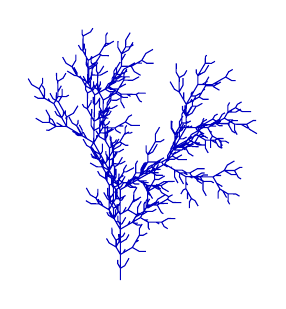
\begin{tikzpicture} 
\draw [blue!75!black, rotate=90]
[l-system={rule set={F -> FF-[-F+F]+[+F-F]}, axiom=F, order=4, step=2pt, 
randomize step percent=25, angle=30, randomize angle percent=5}]
lindenmayer system; 
\end{tikzpicture}
\\
\today
}
\title{Lesson 6: Homogeneous First-Order Equations}

\begin{document}

\frame{\titlepage}

\section{What do we know?}
\begin{frame}\frametitle{What do we know?}
\begin{columns}[T]
\begin{column}{0.6\linewidth}
\begin{itemize}[<+-|alert@+>]
\item The concepts of differential equation and \textbf{initial value problem}
\begin{equation*}
F\big(x,y,y',\dotsc,y^{(n)}\big)=0
\end{equation*}
\item The concept of \textbf{order} of a differential equation.
\item The concepts of \textbf{general solution}, \textbf{particular solution} and \textbf{singular solution}.
\item Slope fields
\item Approximations to solutions via \textbf{Euler's Method} and \textbf{Improved Euler's Method}
\end{itemize} 
\end{column}
\begin{column}{0.4\linewidth}
\begin{itemize}[<+-|alert@+>]
\item Separable equations $y'=H_1(x) H_2(y)$
\end{itemize}
\end{column}
\end{columns}
\end{frame}

\section{Homogeneous First-Order Equations}
\subsection{Definition}
\begin{frame}\frametitle{Homogeneous First-Order Equations}
\framesubtitle{Definition}
A \alert{homogeneous first-order equation} is one that can be written in the form
\begin{equation*}
y'=H\big( \tfrac{y}{x} \big)	
\end{equation*}
\pause To solve them, we always attempt first the substitution $v=y/x$, which turns them into \emph{separable equations}:
\begin{columns}[T]
\begin{column}{0.45\linewidth}
\begin{align*}
\uncover<2->{v&=\frac{y}{x} \\}
\uncover<3->{xv &= y \\}
\uncover<4->{\frac{d}{dx} \big( xv \big) &= \frac{d}{dx}\big( y \big) \\}
\uncover<5->{\alert<7>{v + x \frac{dv}{dx}} & \alert<7>{= \frac{dy}{dx}}}
\end{align*}
\end{column}
\only<6->{\vrule{}}
\begin{column}{0.45\linewidth}
\begin{align*}
\uncover<6->{\alert<7>{\frac{dy}{dx}} &=H\big(\tfrac{y}{x} \big)\\}
\uncover<7->{v + x \frac{dv}{dx} &= H(v) \\}
\uncover<8->{x \frac{dv}{dx} &= H(v)-v \\}
\uncover<9->{\alert{\frac{dv}{H(v)-v}} &\alert{= \frac{dx}{x}}}
\end{align*}	
\end{column}
\end{columns}
\end{frame}

\subsection{Examples}
\begin{frame}\frametitle{Homogeneous First-Order Equations}
\framesubtitle{Examples}
\begin{example}
Find a general solution to the equation
\begin{equation*}
y'=\big( \tfrac{y}{x} \big)^2 + \tfrac{y}{x}	
\end{equation*} 	
\end{example} 
\pause Let us perform the substitution from scratch (it is easier!):
\begin{align*}
v &=\frac{y}{x} &\frac{dy}{dx} &=v+x \frac{dv}{dx} 
\end{align*}
\pause In our equation, this gives us
\begin{columns}[T]
\begin{column}{0.45\linewidth}
\begin{align*}
\uncover<3->{\frac{dy}{dx} &= \big( \tfrac{y}{x} \big)^2 + \tfrac{y}{x} \\}
\uncover<4->{v + x\frac{dv}{dx} &= v^2 + v\\}
\uncover<5->{x\frac{dv}{dx} &= v^2}
\end{align*}
\end{column}
\begin{column}{0.45\linewidth}
\begin{align*}
\uncover<6->{\only<7->{\int} v^{-2}\, dv &= \only<7->{\int} \frac{dx}{x} \\}
\uncover<8->{\alert<8>{-v^{-1}} &\alert<8>{= \ln \lvert x \rvert + C}\\}
\uncover<8->{\alert{-\frac{x}{y}} &\alert{= \lvert x \rvert + C}}
\end{align*}
\end{column}
\end{columns}
\end{frame}

\begin{frame}\frametitle{Homogeneous First-Order Equations}
\framesubtitle{Examples}
\begin{example}
Find a general solution to the equation	
\begin{equation*}
\frac{dy}{dx} = \frac{y}{x} + e^{y/x}	
\end{equation*}
\end{example} 
\begin{align*}
\uncover<2->{\frac{dy}{dx} &= \frac{y}{x} + e^{y/x}} \uncover<5->{&\only<6->{\int} e^{-v}\, dv &= \only<6->{\int} \frac{dx}{x}} \\
\uncover<3->{v+x \frac{dv}{dx} &= v + e^v} \uncover<7->{&-e^{-v} &= \ln \lvert x \rvert + C} \\
\uncover<4->{x \frac{dv}{dx} &= e^v} \uncover<8->{&\alert{-e^{-y/x}} &\alert{=\ln \lvert x \rvert + C}}
\end{align*}
\end{frame}

\begin{frame}\frametitle{Homogeneous First-Order Equations}
\framesubtitle{Examples}
\begin{example}
Find a general solution to the equation
\begin{equation*}
2xy \frac{dy}{dx} = 4x^2 + 3y^2	
\end{equation*}	
\end{example}    
\pause Our first step \alert{always} with first-order differential equations is to write them down in the form $y'=H(x,y)$, whenever possible.
\begin{equation*}
\alert{\frac{dy}{dx}} = \frac{4x^2+3y^2}{2xy} = \frac{4x^2}{2xy} + \frac{3y^2}{2xy}	= \alert{2\frac{x}{y} + \frac{3}{2} \frac{y}{x}}
\end{equation*}
\pause We proceed to perform the substitution now:
\begin{equation*}
v+ x\frac{dv}{dx} = 2v^{-1}+\frac{3}{2}v	
\end{equation*}
\end{frame}

\begin{frame}\frametitle{Homogeneous First-Order Equations}
\framesubtitle{Examples}
\begin{example}
Find a general solution to the equation
\begin{equation*}
2xy \frac{dy}{dx} = 4x^2 + 3y^2	
\end{equation*}	
\end{example}    
And we continue as before:
\begin{align*}
v+ x\frac{dv}{dx} &= 2v^{-1}+\frac{3}{2}v \uncover<6->{&\int \frac{2v}{4+v^2}\, dv &= \int \frac{dx}{x} }\\
\uncover<2->{x\frac{dv}{dx} &= 2v^{-1} + \frac{1}{2}v} \uncover<7->{&\ln (4+v^2) &= \ln \lvert x \rvert + C}\\
\uncover<3->{\only<4->{\int} \frac{dv}{2v^{-1}+ \frac{1}{2}v} &= \only<4->{\int} \frac{dx}{x}} \uncover<8->{&4+v^2 &= A\lvert x \rvert} \\
\uncover<5->{\int \frac{dv}{\frac{4+v^2}{2v}} &= \int \frac{dx}{x}} \uncover<9->{&\alert{4+\big(\tfrac{y}{x}\big)^2} &\alert{= A \lvert x \rvert}}
\end{align*}
\end{frame}
\end{document}